%\UseRawInputEncoding
\documentclass{article}
\setcounter{secnumdepth}{0}
\usepackage[T1]{fontenc}
\usepackage[utf8]{inputenc}
%\usepackage[latin1]{inputenc}
%\usepackage[english, norsk]{babel}
\usepackage{filecontents}
\usepackage{tcolorbox}
\usepackage{url}
\usepackage{etoolbox}
\usepackage{framed}
\usepackage{framed, color}
\usepackage{xcolor}
\usepackage{mdframed}
\usepackage{float}
\usepackage{gensymb}
\usepackage{amsmath}

\definecolor{Black}{rgb}{0.0, 0.0, 0.0}

%Definer kode
\usepackage{listings}
\usepackage{color}
\definecolor{dkgreen}{rgb}{0,0.6,0}
\definecolor{gray}{rgb}{0.5,0.5,0.5}
\definecolor{mauve}{rgb}{0.58,0,0.82}

\lstset{frame=tb,
extendedchars = true,
texcl=true,
  language=C++,
  aboveskip=3mm,
  belowskip=3mm,
  showstringspaces=false,
  columns=flexible,
  basicstyle={\small\ttfamily},
  numbers=none,
  numberstyle=\tiny\color{gray},
  keywordstyle=\color{blue},
  commentstyle=\color{dkgreen},
  stringstyle=\color{mauve},
  breaklines=true,
  breakatwhitespace=true,
  tabsize=3
}

\usepackage[colorlinks]{hyperref}
\hypersetup{citecolor=Black}
\hypersetup{linkcolor=Black}
\hypersetup{urlcolor=Black}
\usepackage{cleveref}


\setlength{\parindent}{0em}
\setlength{\parskip}{1em}
%\renewcommand{\baselinestretch}{2.0}

%\renewcommand\thesubsection{\alph{subsection}}

\renewcommand{\figurename}{Figure}
\begin{document}
\author{Kent Odde}
\title{Introduction to Cybersecurity, Assignment 1}

\maketitle

\newpage

\tableofcontents

\newpage

\section{Abstract}

%Innholdsfortegnelse
\section{Q1}

\textbf{CIA - Confidentiality, Integrity and Availability.}

Alice wants to send the message "Introduction to Data and Cyber-Security (DCS3101)" to Bob. If she wants to employ the CIA concepts in the sending of this message, she has to ensure three things:
\begin{itemize}
\item{\textbf{Confidentiality}: She will have to make sure that Bob is the only one that will be able to read the contents, and that all other third parties will not.}
\item{\textbf{Integrity}: This means making sure that Bob can be certain that the message he receives is in fact the intended message communicated by Alice. Simply put, he needs to know that the contents has not been altered in any way.}
\item{\textbf{Availability}: All the security in the world is meaningless if Bob is not able to decrypt the message. The correct contents of the message must be available for the intended receiver, at the right time.}
\end{itemize}

These three properties are by no means independent, and one will always have to analyze ones needs, and do a trade-off analysis between the three.

High confidentiality and integrity may lead to lowered availability. Either in terms of time it takes to decrypt the message or the complexity of it. In the extreme case, the confidentiality and integrity is so high that the availability is equal to zero. On the other hand a high emphasis on availability may compromise the level of confidentiality and integrity. 

%Oppgaven
\section{Q2}
\subsection{Illustration of Vignere Ciphering}

In order to explain Vignere ciphering, we have to realize that Vignere ciphering is nothing more than an an expanded and enhanced version of Ceasar ciphering. Let's start off by explaining a Ceasar Cipher. 

Ceasar Cipher is a ciphering scheme where we apply an operation to all of the characters in a string. This may be shifting each character by +5 places. In this case we say that the key is F, as it is the letter with the value of 5, given that we count A as 0.

\begin{figure}[H]
 \centering
  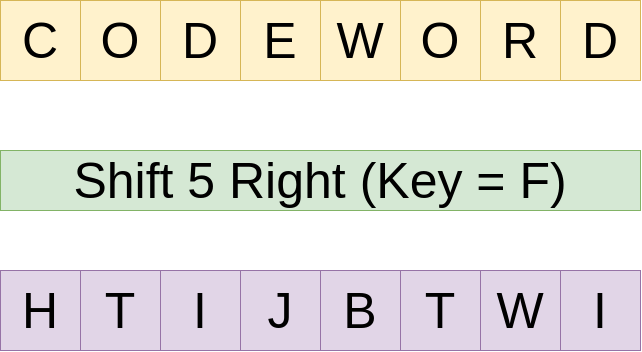
\includegraphics[width=200pt]{img/ceasar.png}
 \caption{Simple Ceasar cipher example}
 \end{figure}

There are many flaws in this scheme, where the most obvious one is that the operation is static, and if you crack one character, you crack all of them. A statistical attack can be very effective here.

\begin{figure}[H]
 \centering
  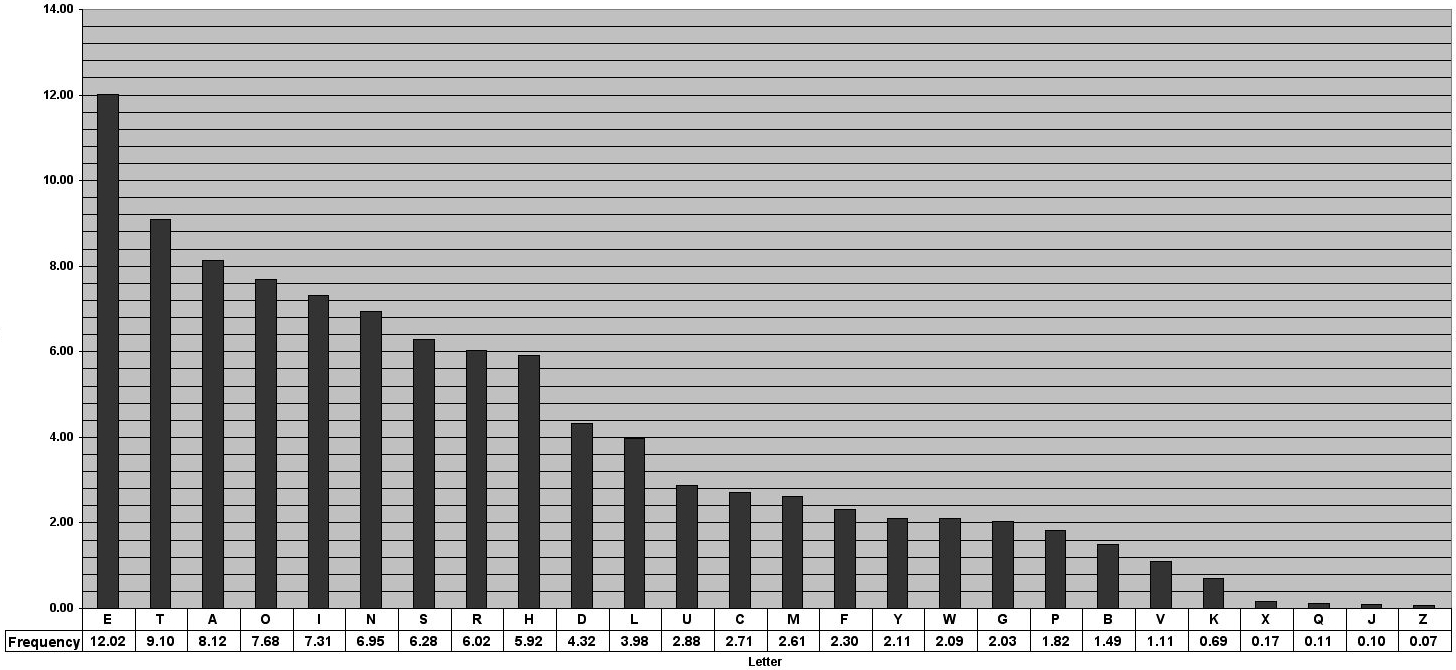
\includegraphics[width=300pt]{img/frequency.jpg}
 \caption{English letter frequency\cite{LETTER}}
 \end{figure}

In this graph we see that the most common letters in the english language are E, T, A and O. If we assume this is also true for our ciphertex HTIJBTWI, we can guess that either the T or the I will map to one of these letters. If we start at the top with the letter I, we will only need to test 4 operations, before arriving at the correct one. 

A vignerecipher attemps to increase the complexity of the Ceasar Cipher by having the operations change for each character. 

Instead of having a key like F in the caesarcipher, we use a key where the number of characters is greater than one. The length of the key naturally increases the robustness of the encryption. 

\begin{figure}[H]
 \centering
  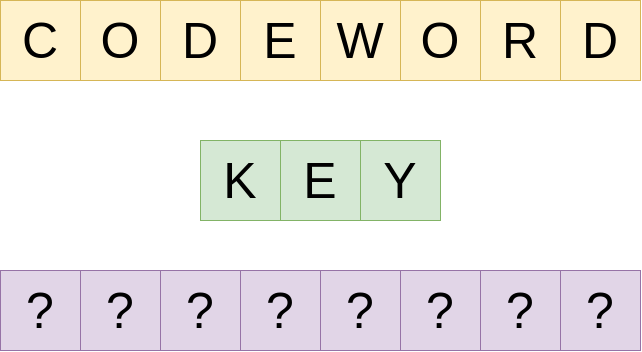
\includegraphics[width=300pt]{img/vigneredraw1.png}
 \caption{Vignere 1}
 \end{figure}

In the example where the key is 'KEY', we use the key 'K' on the first character of the plaintext string, 'E' is the key off the second, and so on. When we reach the last character of the Key, we start over, so that the 4th character of our plaintext will also be encrypted with the key 'K'.

\begin{figure}[H]
 \centering
  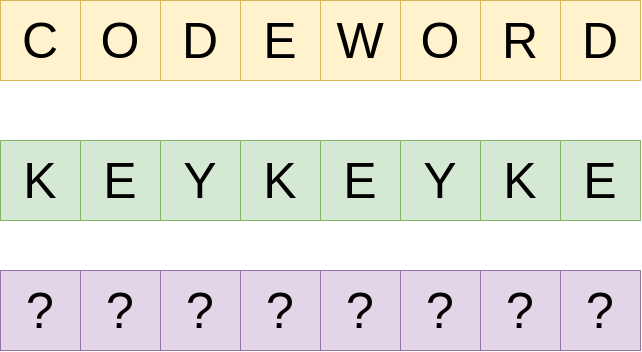
\includegraphics[width=300pt]{img/vigneredraw2.png}
 \caption{Vignere 2}
 \end{figure}

In the following figure, we can see that the two O's and the two D's not longer map to the same letter, as was the problem with the Ceasar Cipher. In the ciphertext we can also see a couple of examples where two equal letters, like M and B, map back two different letters in the plaintext. 

\begin{figure}[H]
 \centering
  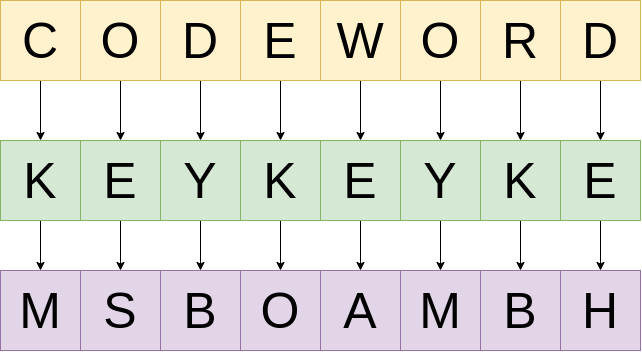
\includegraphics[width=300pt]{img/vigneredraw3.png}
 \caption{Vignere 3}
 \end{figure}



If the message is shorter than the key, or if the key is not a multiple of the message (like in the example), we may add padding to the plaintext before encrypting. This is a mechanism of making the messages harder to diciphire, because the length of the ciphertext, does not necessarily match the length of the plaintext. The padding should not however consist of the same character. If one tries to shift the last few characters through the alphabet, the key may become obvious from this. As an illustration, let us imagine padding the message with the letter A. 

\begin{figure}[H]
 \centering
  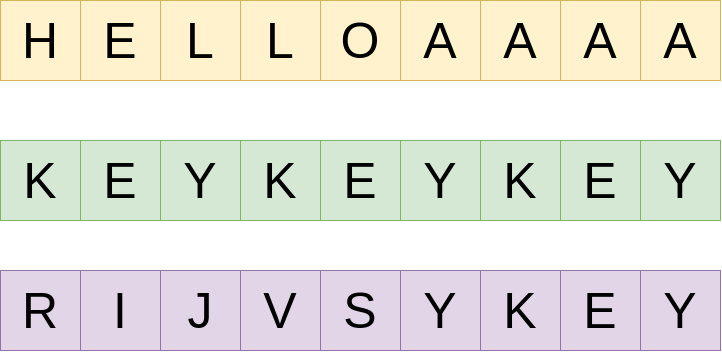
\includegraphics[width=300pt]{img/vigneredraw4.png}
 \caption{A very unfortunate padding scheme}
 \end{figure}

This is of course an extreme example, because A will just give the key in plaintext, but no matter which letter we replace A with, the key will reveal itself after a maximum of 26 shift operations. Because of this, the padding scheme should include either a repetition of some part of the message, or random characters. 

\subsection{Vignere Cipher Program}

When writing the vignere ciphering program, i assumed the following:
\begin{itemize}
\item{Upper case characters will be encrypted within the set of upper case characters}
\item{Lower case characters will be encrypted within the set of lower case characters}
\item{Spaces, commas and periods will not be encrypted and only represent themselves}
\item{Keys are of course case insensitive}
\item{In the part with two keys, I assumed that the purpose is to encrypt the message twice, using two different keys}
\end{itemize}

\subsubsection{Single Key}

The text given in the task, encrypted with the key \textit{kongsberg}, became:
\begin{align*}
Dvr\quad wmjgb\quad hbcjt\quad xpb\quad aawdf\quad unfv\quad kno\quad znfq\quad esx.
\end{align*}

The result can also be seen in the figure below:

\begin{figure}[H]
 \centering
  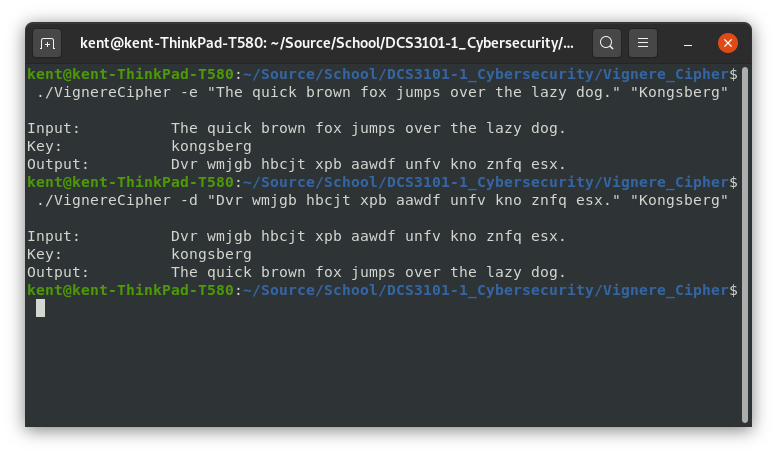
\includegraphics[width=300pt]{img/vignere1key.png}
 \caption{Vignere cipher, 1 key}
 \end{figure}

\subsubsection{Two Keys}



Encrypted twice, with the keys \textit{norway} and \textit{oslo}, became:
\begin{align*}
Ung\quad aiyam\quad gfzio\quad lqh\quad xkkrx\quad cgqs\quad zjo\quad zqxa\quad icr.
\end{align*}

The result can also be seen in the figure below:
\begin{figure}[H]
 \centering
  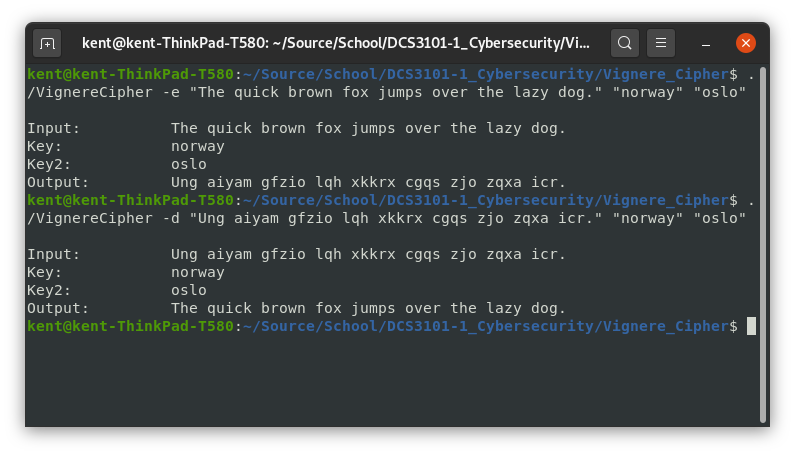
\includegraphics[width=300pt]{img/vignere2keys.png}
 \caption{Vignere cipher, 2 keys}
 \end{figure}

%Implementation
\section{Q3}
Lets start by defining the terms diffusion and confusion.
%Konklusjon
\section{Q4 - Enigma}

In this task, I will assume knowledge about the Enigma machine on the part of the reader, and not go into the details as this would lead to a very extensive task. There are also some conflicting sources of information about the Enigma. I have gathered all data about models, rotors and reflektors from \cite{ENIGMA1} \cite{ENIGMA2}

The Enigma I, had a scheme where one would choose three rotors out of five, and one reflektor out of three. This can be seen in the figure below. 

\textit{Some sources say that the Enigma I had only three rotors and some say five.}

\begin{figure}[H]
 \centering
  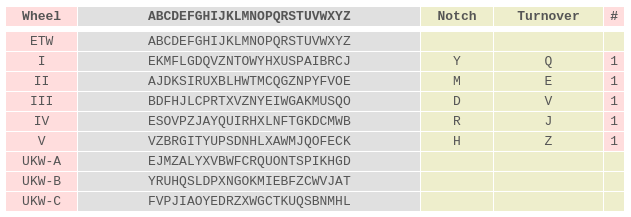
\includegraphics[width=300pt]{img/enigmaIspecs.png}
 \caption{Rotor specifications for Enigma I}
 \end{figure}

To increase the complexity and challenge of this task, I decided implementing an M3 Enigma. This model had a total of eight rotors to choose from, instead of five. However, reflektor-A seemed to be removed. However, in order for this program to be compatible with the Enigma I, I have decided to include all three reflektors. 

\begin{figure}[H]
 \centering
  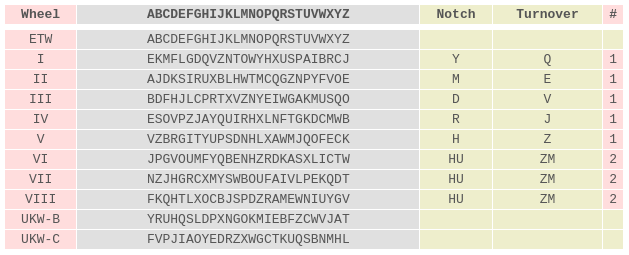
\includegraphics[width=300pt]{img/enigmaM3specs.png}
 \caption{Rotor specifications for Enigma M3}
 \end{figure}

For the most part this is quite a trivial task. When pushing a button, the rotors will increment. The signal will run from the button, through the plugboard, through the rotors, into the reflektor, back through the rotors, back through the plugboard, and deliver an output. In code this will for the most part consist of looking up characters in constant arrays, taking into account the current position of the rotors. 

However the thing that stomped me for a while, were the ringsettings. The ringsettings are not dynamically changed, but are set by twisting the actual rotor relative to itself. This combined with the rotor position made me resort to pen and paper. Finally i was able to come up with a working function for a transformation through a rotor with a certain position and ring setting, which can be seen in rotor.cpp, called getTransformedChar().

In order to test the program properly, I generated correct ciphertexts with several different settings at \url{https://cryptii.com/pipes/enigma-machine}.
\begin{figure}[H]
 \centering
  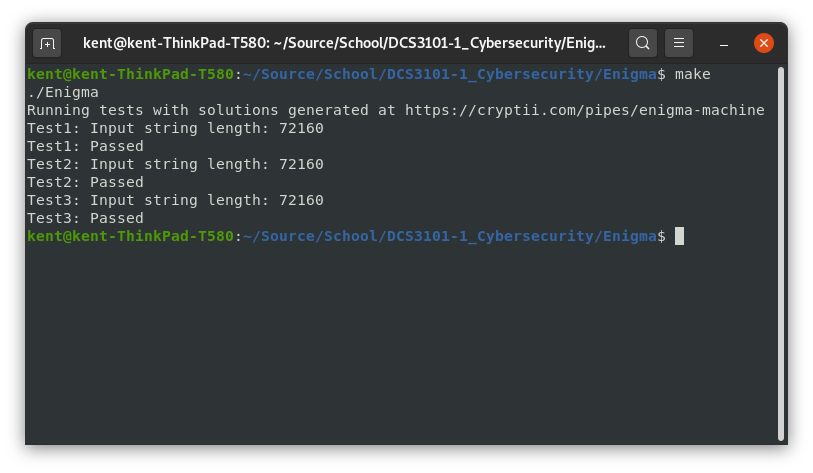
\includegraphics[width=300pt]{img/enigmaTest.png}
 \caption{Test of Enigma}
 \end{figure}
As can be seen in the figure, these strings were quite long in order to go through all the positions several times. These tests will be excluded from the code in the appendix, because of their size.


In the figure below, one can see a string be encrypted, decrypted and a check performed to see that it in fact has returned the correct plaintext back.
\begin{figure}[H]
 \centering
  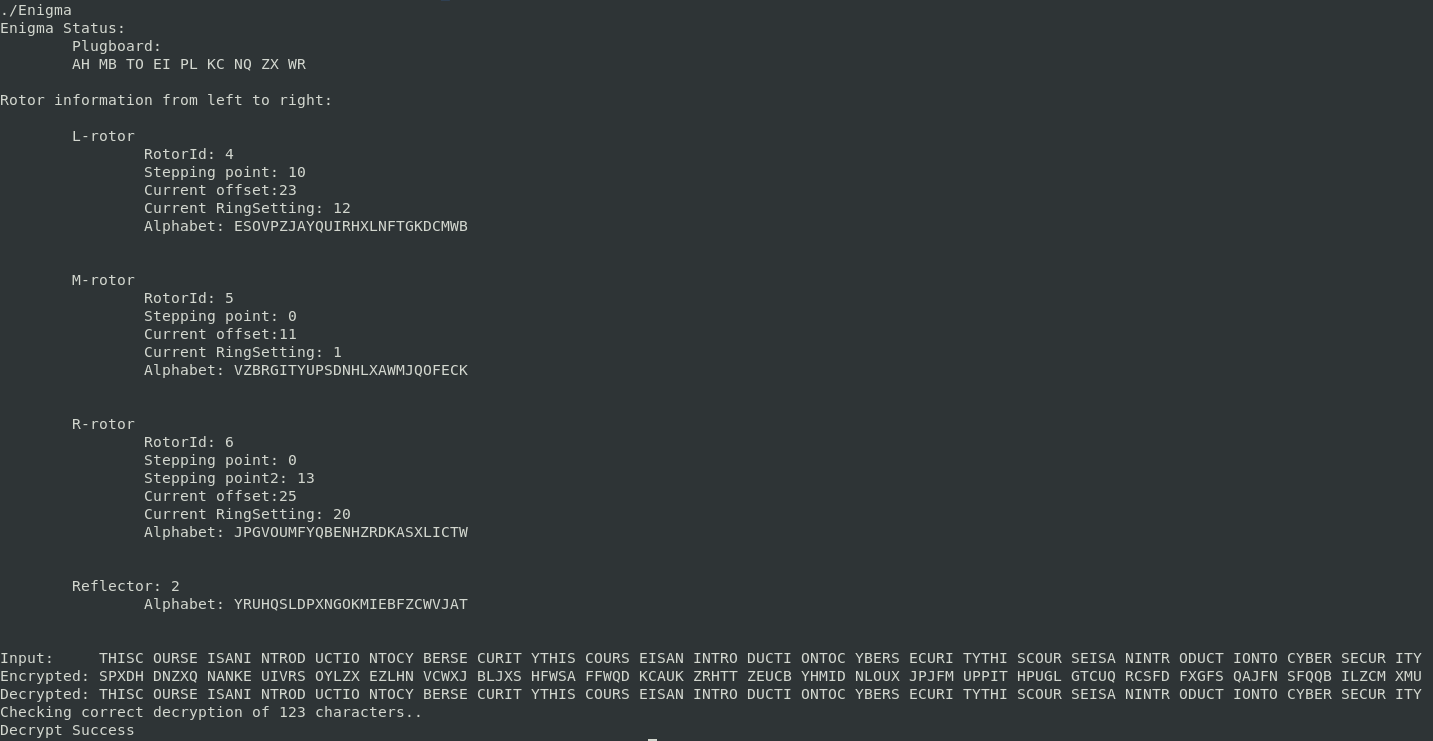
\includegraphics[width=300pt]{img/enigmaMan.png}
 \caption{Enigma}
 \end{figure}




%Vedlegg
\section{Appendices}
\subsection{Vignere Cipher Code}
\begin{lstlisting}
#include <iostream>
#include <string>
#include <algorithm>


int STARTASCIILOWER = 97;
int STOPASCIILOWER = 122;
int STARTASCIIUPPER = 65;
int STOPASCIIUPPER = 90;

/*
As the %-operator does not behave like modulo on negative numbers, this function is necessary
*/
int modulo(int a, int b)
{
	return (a % b + b) % b;
}

char shiftChar(char c,  char shiftBy, bool backward = false)
{	
	/*
	Checking if the characters upper or lower case, and chooses the asciiboundaries of the respective set.
	*/
	int startAscii = (c >= STARTASCIILOWER) ? STARTASCIILOWER : STARTASCIIUPPER;
	int stopAscii = (c >= STARTASCIILOWER) ? STOPASCIILOWER : STOPASCIIUPPER;

	/*
	Move the character downto the 0-25 range, performing the shift, and moving it back up the correct asciirange. 
	*/
	char output = c - startAscii;
	if(backward)
	{
		output = modulo((output - (shiftBy - STARTASCIILOWER)), (stopAscii - startAscii + 1)) + startAscii;
	}
	else
	{
		output = modulo((output + (shiftBy - STARTASCIILOWER)), (stopAscii - startAscii + 1)) + startAscii;
	}
	return output;
}

std::string encrypt(std::string plainText, std::string key)
{
	int keyIndex = 0;
	std::string cipherText;
	for(int i = 0; i < plainText.size(); i++)
	{
		/*
		Dont encrypt spaces, commas and periods.
		*/
		if(plainText[i] == ' ' || plainText[i] == '.' || plainText[i] == ',')
		{
			cipherText += plainText[i];
			continue;
		}
		cipherText += (shiftChar(plainText[i], key.at(keyIndex)));
		keyIndex = (keyIndex + 1) % key.size();
	}
	return cipherText;
}

std::string decrypt(std::string cipherText, std::string key)
{
	int keyIndex = 0;
	std::string plainText;
	for(int i = 0; i < cipherText.size(); i++)
	{
		/*
		Dont decrypt spaces, commas and periods.
		*/
		if(cipherText[i] == ' ' || cipherText[i] == '.' || cipherText[i] == ',')
		{
			plainText += cipherText[i];
			continue;
		}

		plainText += (shiftChar(cipherText[i], key.at(keyIndex), true));
		keyIndex = (keyIndex + 1) % key.size();
	}
	return plainText;
}


int main(int argc, char* argv[]) 
{
	/*
	Mostly commandline argument handling
	*/
	if(argc < 4)
	{
		std::cout << "Wrong number of arguments passed\n";
		std::cout << "Arguments: \n\t./Vignere cipher -e/d <string> <key> <optionalSecondKey>\n";
		return -1;
	}

	std::string input = argv[2];
	std::string key = argv[3];
	std::transform(key.begin(), key.end(), key.begin(), ::tolower);
	std::string key2 = "";
	if(argc > 4)
	{	
		key2 = argv[4];
		std::transform(key2.begin(), key2.end(), key2.begin(), ::tolower);
	}
	std::string output;

	if(std::string(argv[1]) == "-e")
	{
		output = encrypt(input, key);

		if(key2.compare("") != 0)
		{
			output = encrypt(output, key2); 
		}
	}
	else if(std::string(argv[1]) == "-d")
	{
		output = decrypt(input, key);

		if(key2.compare("") != 0)
		{
			output = decrypt(output, key2);
		}
	}
	else
	{
		std::cout << "Error, expected arguments:\n\t/Vignere cipher -e/d <string> <key> <optionalSecondKey>\n";

		return -1;
	}
	std::cout << "\nInput:\t\t" << input << "\n";
	std::cout << "Key:\t\t" << key << "\n";
	if(key2.compare("") != 0) std::cout << "Key2:\t\t" << key2 << "\n";
	std::cout << "Output:\t\t" << output << "\n"; 
	return 0;
}
\end{lstlisting}

\subsection{Enigma Code}
\subsubsection{main.cpp}

\subsubsection{Enigma Class}

\subsubsection{Rotor Class}




\newpage
%Referanse
%\section{Referanser}

\nocite{*}
\bibliographystyle{plain}
\bibliography{ref}

\addcontentsline{toc}{section}{References}

\end{document}